\documentclass[british]{beamer}

\usepackage{default}
\usepackage[british]{babel}
\usepackage{epstopdf}
\usetheme{Madrid}
\usepackage{graphicx}
\usepackage{dirtytalk}
\usepackage{csquotes}
\usepackage{wrapfig}
\usepackage{tikz}
\usepackage{smartdiagram}

\begin{document}
%
\title[Document Semantic Similarity]
{Document Semantic Similarity}

\subtitle{TIS Project}

\author[A. Pirovano, F. Picciotti]
{Alberto Pirovano \and Francesco Picciotti}

\institute[PoliMi]
{
	Politecnico di Milano
}

\logo{
	
\includegraphics[height=1.7cm,trim={0 2cm 4.5cm 2cm},clip]
	{./Imgs/Politecnico-di-Milano-3-m8qw.eps}
	}	

\AtBeginSection[]
{
	\begin{frame}
		\frametitle{Outline}
		\tableofcontents[currentsection, currentsubsection]
	\end{frame}
}

\AtBeginSubsection[]{
	\begin{frame}
		\frametitle{Outline}
		\tableofcontents[currentsection, currentsubsection]
	\end{frame}
}

\maketitle

\section{State of art}

\begin{frame}{Introduzione}
	L'attuale stato dell'arte per similitudine semantica tra documenti si suddivide in:
	\begin{itemize}
		\item NLP Tradizionale
		\item Vector Space Model
		\item Deep Learning based 
	\end{itemize}
\end{frame}
	
\subsection{NLP tradizionale}
	
\begin{frame}{NLP Tradizionale}
	Questo approccio segue la letteratura del Natural Language Processing e consiste dei seguenti passi:
	\begin{itemize}
		\item Cleaning dei dati
		\item Pos-Tagging
		\item Stemming o Lemmatisation
		\item Parsing
		\item Ontologia
	\end{itemize}
	Tuttavia nel caso del nostro scopo presenta delle criticit\`{a}, ovvero:
	\begin{itemize}
		\item Affidabilit\`{a} del Pos-Tagger italiano di TreeTagger
		\item Reperire una Ontologia e un parsing toll nella lingua italiana
	\end{itemize}
\end{frame}

\begin{frame}{NLP Tradizionale}
	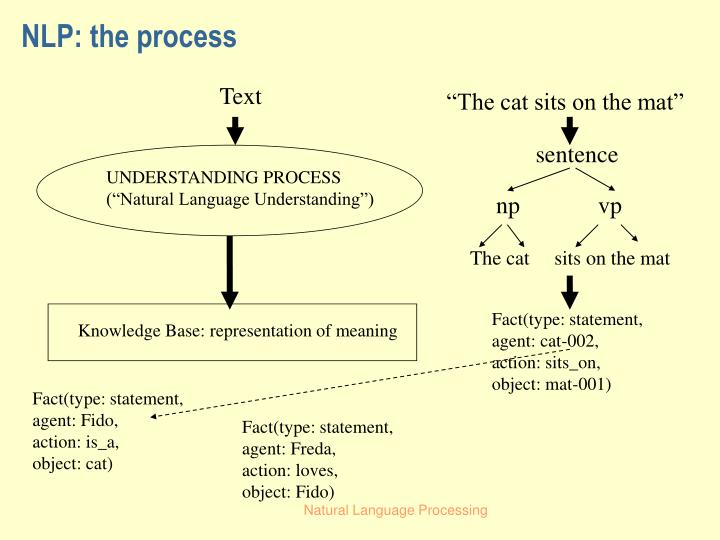
\includegraphics[width=0.9\textwidth, height=0.85\textheight]{./Imgs/nlp-the-process.jpg}
\end{frame}
	
\subsection{Vector Space Model}
	
\begin{frame}{Vector Space Model}
	\begin{wrapfigure}{r}{0.4\textwidth}
		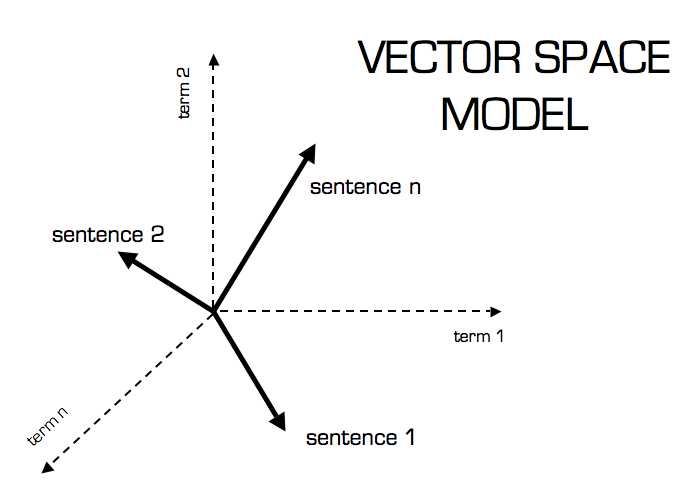
\includegraphics[width=1.1\linewidth,height=0.4\textwidth]{./Imgs/vector_space.png}
	\end{wrapfigure}	
	\`{E} basato sulla rappresentazione vettoriale del documento in un piano dove le diverse dimensioni sono il Bag of Word di tutti i documenti.
	Questo approccio richiede dei seguenti steps:
	\begin{itemize}
		\item Cleaning dei dati
		\item Stemming o Lemmatisation
		\item Encoding del documento in vettore
		\item TF/IDF + LSA (Latent Semantic Analysis)
		\item Similarity (Cosine, Pearson, ...)
	\end{itemize}
\end{frame}
	
\begin{frame}{...limiti?}
	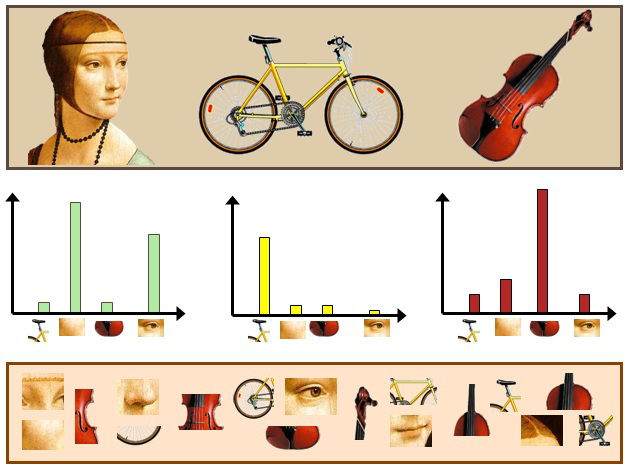
\includegraphics[width=0.9\textwidth, height=0.8\textheight]{./Imgs/bow-example.jpeg}
\end{frame}
	
\begin{frame}{Geometrico: limiti}
	Per riassumere:
	\begin{itemize}
		\item Molto dipendente dal preprocessing del corpus
		\item Grande Bag Of World $\rightarrow$ bisogno di LSA, ma non \`{e} così banale.
		
		Perch\'{e}?
		\begin{displayquote}
			"LSA assumes that words that are close in meaning will occur in similar pieces of text"
		\end{displayquote}
		\item Semantica e ambiguit\`{a}
		\item Un documento \`{e} un insieme \alert{non ordinato} di parole  
	\end{itemize}
\end{frame}
	
\subsection{Deep Learning}
	
\begin{frame}{E non solo}
	\begin{figure}[!hf]
		\centering
		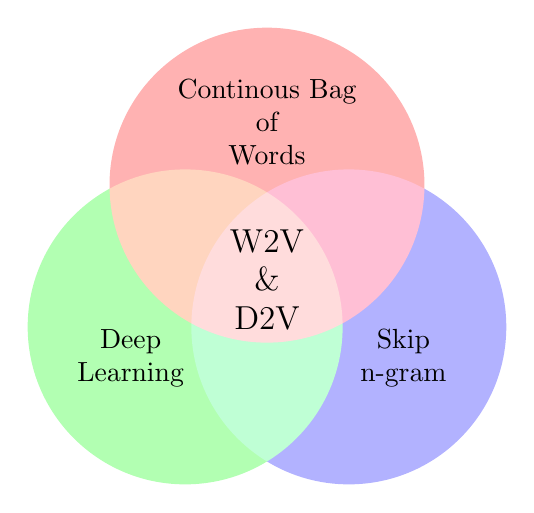
\begin{tikzpicture}
		\begin{scope}[blend group = soft light]
		\fill[red!30!white]   ( 90:1.2) circle (2);
		\fill[green!30!white] (210:1.2) circle (2);
		\fill[blue!30!white]  (330:1.2) circle (2);
		\end{scope}
		\node at ( 90:2)    
		[font= \normalsize, align= center]
		{Continous Bag \\ of \\ Words};
		\node at ( 210:2)   
		[font= \normalsize, align= center]
		{Deep \\ Learning};
		\node at ( 330:2)   
		[font= \normalsize, align= center]
		{Skip \\ n-gram};
		\node [font=\large, , align= center] {W2V \\\& \\D2V};
		\end{tikzpicture}
	\end{figure}
\end{frame}
	
\begin{frame}{Deep Learning: W2V \& D2V}
	Negli ultimi anni il Deep Learning trova numerose applicazioni con ottimi risultati.\par
	La creazione di Word2Vec da Google offre un modello che ha principalmente, i seguenti vantaggi e svantaggi.
	\begin{columns}
		\column{0.5\textwidth}
		\\
		\underline{Pros:}
		\begin{itemize}
			\item Molto meno dipente da un preprocessing
			\item Context-aware
			\item Combina il metodo \textit{Geometrico} con quello \textit{NLP Tradizionale}
			\item Non sfrutta una ontologia, ma la \alert{crea} 
		\end{itemize}
		\column{0.5\textwidth}
		\underline{Cons:}
		\begin{itemize}
			\item Tecnica unsupervised 
			\item Bisogno di un esperto per validare gradi di similarità
			\item Pu\`{o} risultare in GIGO system (Garbage In Garbage Out)
		\end{itemize}
	\end{columns}
\end{frame}
	
\section{Data Preparation}

\begin{frame}{Dataset}
	\begin{displayquote}
		"Preprocessing is 80\% of NLP work"
		 
		\begin{flushright}
			\textit{Lev Konstantinovskiy}
		\end{flushright}
	\end{displayquote}
	Il dataset fornitoci \`{e} composto da due corpus: 
	\begin{itemize}
		\item il corpus del Sole 24 Ore con 3265 articoli, di cui 31 non hanno body
		\item il corpus di Radiocor con 6916 articoli
	\end{itemize}
	Il corpus prima del preprocessing contiene quindi 10150 articoli. \par
	Togliendo i duplicati otteniamo 9283 articoli, cio\'{e} ci sono 867 articoli duplicati.
\end{frame}

\subsection{Preprocessing}

\begin{frame}{Pipeline completa}
	\begin{center}
		\smartdiagramset{
			module minimum width= 5cm, 
			text width= 4.5cm,
			font= \tiny,
			set color list={blue!50!cyan,green!60!lime,orange!50!red,red!80!black},
			back arrow disabled=true}
		\smartdiagram[flow diagram: horizontal]{Cleaning del testo,Tokenizzazione e rimozione punteggiatura, Rimozione stopwords e POS-tagging del testo,Lemmatizzatione,Merge di verbi passivi composti}
	\end{center}
\end{frame}

\subsection{Cleaning del testo}

\begin{frame}{Cleaning pipeline}
	\begin{center}
			\smartdiagramset{
				module minimum width= 5cm,
				module minimum height= 0.1cm, 
				text width= 5cm,
				module y sep= 0.8cm,
				font= \tiny,
				set color list={blue!50!cyan,green!60!lime,orange!50!red,red!80!black},
				back arrow disabled=true}		
			\smartdiagram[flow diagram: vertical]{Lowercase di ogni lettera, Escape di caratteri unicode non printabli, Tokenizzazione numeri percentuali, Rimozione preposizioni contratte, Tokenizzazione parola s24, Unificazione di espressioni di quantità, Rimozione di intestazione di articolo, Rimozione di interruzione pagina, Rimozione chiusura aricolo, Rimozione urls e tags html}
	\end{center}
\end{frame}

\section{Word2Vec}

\begin{frame}{Hello}
	Qui speghiamo per bene come funziona word2vec
\end{frame}

\section{Doc2Vec}

\begin{frame}{Hello}
	Qui speghiamo per bene come funziona word2vec
\end{frame}
\end{document}
